\chapter{Analysis: Turning Intuition into Reliable Theorems}

\section{A Strange Question on a Mountain Path}

During the summer holidays, your family climbs a mountain. The foot is $100$ metres above sea level and the summit $1500$ metres. You leave at eight in the morning and arrive at half past twelve, stopping for rests and even backtracking to find a dropped hat. Your speed changes constantly, with no regular pattern.

Back home, someone asks a strange question: can you guarantee that at some instant during the climb, your altitude was exactly $618$ metres?

Intuitively you say yes. Altitude changes continuously from $100$ to $1500$ metres; surely you cannot jump from $617$ to $619$ metres.

The intuition sounds airtight. Before agreeing too quickly, consider two more questions:

\begin{itemize}
  \item Your record shows an altitude of $500$ metres at nine and $800$ metres at eleven. Must some moment have had altitude exactly $600.001$ metres?
  \item A thermometer rises from $10^\circ$C at dawn to $25^\circ$C at noon. Must the temperature at some instant have been exactly $\sqrt{500}$ degrees Celsius? Remember that $\sqrt{500}$ has a nonterminating, nonrepeating decimal expansion, unreadable on any thermometer's scale.
\end{itemize}

You may still answer yes to the first, but with less confidence: can altitude really be discussed with infinite precision? The second is harder. How can a value no thermometer can display have been passed through exactly?

This chapter forges the feeling that continuous change skips no intermediate value into a theorem that can be proved and trusted. The craft is \textbf{analysis}: its aim is to make intuition reliable, rather than merely speed up calculation. Mathematicians spent two centuries on it, having been fooled repeatedly by their intuitions, sometimes spectacularly.

\section{Intuition Is Fooled for the First Time}

The simplest picture of continuity is a graph drawable without lifting a pencil. Useful, but unreliable: historically it failed in at least three ways.

First, if skipping no intermediate value seems obvious, consider
\[
f(x)=\begin{cases}1, & x\ge 0,\\ -1, & x<0.\end{cases}
\]
It takes value $-1$ at $x=-1$ and $1$ at $x=1$, but never the intermediate value $0$. The graph jumps at $x=0$. Passing through intermediate values really does depend on the no-jumps condition.

Second, something subtler: since $1^2=1<2$ and $2^2=4>2$, the solution $\sqrt{2}$ of $x^2=2$ ought to be passed through between $1$ and $2$. Yet $\sqrt{2}$ is irrational. In a world containing only rational numbers, $f(x)=x^2-2$ is negative at $x=1$ and positive at $x=2$, but \textbf{never equals zero over the rationals}. The supposedly encountered middle value has no place to occur. Here intuition fails because \textbf{the number system itself has holes}. The rationals resemble a shirt full of pinholes: seemingly complete until inspected closely.

\begin{fanli}
Warning 1: over the rationals, $f(x)=x^2-2$ changes from negative to positive without reaching zero. Half the intermediate value theorem's secret belongs to the function, the other half to the real numbers. Their lack of holes is completeness.

Warning 2: continuous graphs need not be smooth. Weierstrass constructed a function continuous everywhere with no tangent anywhere, an eternally bristly curve that never magnifies into a line. It needs no pencil lift yet has no smooth point. Continuity is much weaker and subtler than smoothness.
\end{fanli}

Third, even without jumps or holes in the numbers, infinity can defeat intuition. The function $g(x)=1/x$ behaves well at every point of $(0,1]$, yet as $x$ approaches $0$, $g(x)$ grows without bound. A finite horizontal range contains unbounded height. The intuition that a finite stretch of curve must have a highest point fails again.

All three failures teach the same lesson: every statement in analysis must withstand the most searching objection. Let us repair the gaps one by one.

\section{Making Continuity Precise}

Repair the first gap: what exactly is continuity? We want \textbf{small input changes to produce small output changes}. More precisely:

\begin{dingyi}[Continuity: An Intuitive Version]
A function $f$ is \textbf{continuous} at $a$ if $f(x)$ approaches $f(a)$ as $x$ approaches $a$. Whatever output-error requirement you choose, such as deviation below $0.001$, there is a small input interval around $a$ in which every $x$ gives an output meeting your requirement. Continuity on an interval means continuity at every point of it.
\end{dingyi}

Notice the challenge structure: \textbf{you} choose the tolerance, however severe, and I \textbf{must} provide a response. A feeling of closeness becomes a testable agreement. The jump function $f(x)$ fails at $x=0$. Demand output deviation below $1/2$; however tightly I restrict inputs near $0$, positive and negative inputs remain, giving outputs $1$ and $-1$, a difference of $2$ that exceeds the demand.

\begin{shuyu}{Continuous Function}
\textbf{Intuition}: a graph drawn without lifting the pencil; small input tremors cause only small output tremors.

\textbf{Formal statement}: as $x$ tends to $a$, $f(x)$ tends to $f(a)$, so the limit equals the function value.

\textbf{Example}: $f(x)=x^2$ is continuous everywhere, since $x$ near $a$ makes $x^2$ near $a^2$. The jump function is discontinuous at $x=0$.
\end{shuyu}

The reals repair the second gap. Their precious property is that \textbf{every process approaching a position arbitrarily closely finds that position among the real numbers}. This is \textbf{completeness}. The rationals lack it: $1,\ 1.4,\ 1.41,\ 1.414,\ \dots$ approaches $\sqrt{2}$, but $\sqrt{2}$ is not rational. The reals have no such defect. Once we accept this, intuition's central claim can be proved.

\section{The Intermediate Value Theorem: No Jumps, No Skipped Values}

\begin{dingli}[The Intermediate Value Theorem]
Suppose $f$ is continuous on $[a,b]$, with $f(a)<0$ and $f(b)>0$, or conversely. Then there is at least one point $c$ in the interval with $f(c)=0$.
\end{dingli}

More generally, $f$ takes every value between $f(a)$ and $f(b)$. Altitude changing continuously from $100$ to $1500$ metres must pass exactly through $618$ metres, and even through the altitude corresponding to $\sqrt{500}$ metres.

The proof resembles binary search in computing: repeatedly halve the suspect interval, leaving the zero nowhere to escape.

\begin{proof}
Suppose $f(a)<0<f(b)$. Examine the midpoint $m_1=(a+b)/2$. If $f(m_1)=0$, we have found the zero. If $f(m_1)>0$, the zero must lie in the left half $[a,m_1]$; if $f(m_1)<0$, in the right half $[m_1,b]$. Either way, we obtain a half-length interval with negative value at the left and positive value at the right.

Repeat. After step $n$, the suspect interval has length $(b-a)/2^n$, with left endpoint $a_n$ satisfying $f(a_n)\le 0$ and right endpoint $b_n$ satisfying $f(b_n)\ge 0$. The sequence $a_1,a_2,a_3,\dots$ is nondecreasing and bounded above by $b$; the right endpoints are nonincreasing and bounded below by $a$. The gap tends to $0$. Completeness gives both endpoint sequences the same limiting position $c$.

Finally use continuity: as $x$ tends to $c$, the values tend to $f(c)$. All left-endpoint values are at most $0$, so their limiting value $f(c)$ is at most $0$. All right-endpoint values are at least $0$, so $f(c)$ is at least $0$. Together these force $f(c)=0$.
\end{proof}

\begin{center}
\begin{tikzpicture}[scale=0.9]
  \draw[->] (-0.3,0) -- (7,0) node[right] {$x$};
  \draw[->] (0,-2.2) -- (0,2.6) node[above] {$y$};
  \draw[thick,domain=0.6:6.2,smooth] plot (\x, {0.6*\x-1.2+0.3*sin(2*\x r)});
  \draw[dashed] (0.6,0) -- (6.2,0);
  \fill (2.5,0) circle (1.5pt) node[below right] {$c$};
  \node[below] at (0.6,-0.65) {$a$};
  \node[above] at (6.2,2.5) {$b$};
  \node[left] at (0,2.2) {$f(b)>0$};
  \node[left] at (0,-1.6) {$f(a)<0$};
\end{tikzpicture}
\end{center}

Look again at the proof: it establishes \textbf{existence} and also \textbf{calculates} the zero. Each cut halves the error; twenty reduce it to about a millionth. For $\sqrt{2}$, start from $1^2<2<2^2$. The midpoint $1.5$ has square $2.25>2$, so take the left half; $1.25$ has square $1.5625<2$, so take the right half. After ten steps you have $1.414$, matching manual square-root calculation. Analysis's first theorem immediately becomes a calculator.

\section{Highest Points and Uniform Temperaments}

The intermediate value theorem governs values in between; its sibling governs extreme values.

\begin{dingli}[The Extreme Value Theorem]
A continuous function on a closed interval $[a,b]$ attains both a maximum and a minimum. There are points $p$ and $q$ in the interval such that $f(p)$ is at least every function value and $f(q)$ at most every function value.
\end{dingli}

Both hypotheses matter. The function $g(x)=1/x$ is continuous on $(0,1]$, but that interval is not closed and there is no maximum. A discontinuous function on a closed interval can jump away from its highest prospective value. This theorem underpins optimization: asking for least material or greatest profit makes sense because suitable functions on suitable domains have answers. Finding them is Chapter 10's work for derivatives.

A finer concept, less common in exams but central to analysis, is \textbf{uniform continuity}. Ordinary continuity gives each point its own response to a tolerance. Uniform continuity requires \textbf{one response for the whole interval}: after you set an output tolerance, I produce a single input-length ruler that works wherever it is placed in the interval.

Why might this fail? For $g(x)=1/x$ on $(0,1]$, the curve becomes steeper near $0$. An input gap of $0.001$ changes output by about $0.001$ near $x=1$, but by thousands near $x=0.001$. Any fixed ruler eventually fails farther left. By contrast, $f(x)=x^2$ behaves well on every \textbf{closed} interval $[a,b]$: its slope is bounded by $2$ times the larger endpoint's absolute value, so a uniform rule is available. Every continuous function on a closed interval can be proved uniformly continuous. Intuition says that a finite stage cannot host infinite unruliness; this time it wins, but only with proof.

\section{Cauchy Sequences: Proving an Answer Exists Before Knowing It}

A deeper question hides in the bisection proof. We construct $a_1,a_2,\dots$ and claim that it approaches some position $c$. But $c$ is what we seek. How can we know it exists \textbf{before} finding it? Could the sequence approach an empty position, like rationals approaching $\sqrt{2}$?

The nineteenth-century mathematician Cauchy gave an elegant answer: \textbf{we need not know the destination in advance} to decide convergence. We need only inspect how closely the sequence's terms stick together.

\begin{dingyi}[Cauchy Sequence: An Intuitive Version]
A sequence $a_1,a_2,a_3,\dots$ is \textbf{Cauchy} if, for any specified tolerance, the distance between \textbf{any two terms} sufficiently far along is no greater than that tolerance.
\end{dingyi}

Every convergent sequence is Cauchy: terms gathering around one destination necessarily gather near each other. The deeper converse asks whether gathering terms always have a destination. Not among rationals: approximations to $\sqrt{2}$ refute it. Among reals, \textbf{they always do}. Every real Cauchy sequence converges: this standard formulation of completeness is analysis's foundation stone.

\begin{shuyu}{Cauchy Sequence}
\textbf{Intuition}: a sequence whose later members cluster as closely together as demanded.

\textbf{Formal statement}: for every tolerance $\varepsilon>0$, there is a term after which the difference between any two terms is less than $\varepsilon$.

\textbf{Example}: $1,\ 1.4,\ 1.41,\ 1.414,\ \dots$, the successive decimal truncations of $\sqrt{2}$, is Cauchy. Beyond decimal place $n$, any two terms differ by at most $10^{-n}$. Its destination is $\sqrt{2}$, a limit available among reals but not rationals.
\end{shuyu}

We now have a new answer to whether an equation has a solution: construct increasingly close approximate solutions, use completeness to guarantee a limit, then continuity to verify that it solves the equation. This procedure proves existence for many equations even when no exact expression for the solution can ever be written.

\section{Power Series: Functions as Infinitely Long Polynomials}

The preceding sections defended intuition by repairing its gaps; the next three use infinite processes to create remarkable new objects. You have already glimpsed the first tool in infinite decimals. The expansion $\pi=3.14159\dots$ splits $\pi$ into $3$ plus $0.1$ plus $0.04$ and further corrections. Power series do the same for \textbf{functions}.

The simplest example is geometric summation. We know $1+x+x^2+\cdots+x^n=\dfrac{1-x^{n+1}}{1-x}$. For $|x|<1$, the term $x^{n+1}$ tends to $0$, giving
\[
\frac{1}{1-x}=1+x+x^2+x^3+\cdots \qquad(|x|<1).
\]
Check $x=1/2$: the right side is $1+1/2+1/4+\cdots=2$, and the left is $1/(1-1/2)=2$. They agree.

Read this in a new way: $\frac{1}{1-x}$ equals an infinitely long polynomial. Why split it this way? Polynomials need only addition and multiplication. Decomposing a difficult function into powers gives a recipe whose number of terms can be chosen to match the required accuracy.

The best-known recipe belongs to the exponential:
\[
e^x=1+x+\frac{x^2}{2!}+\frac{x^3}{3!}+\frac{x^4}{4!}+\cdots
\]
It holds for \textbf{all} $x$, unlike $\frac{1}{1-x}$, whose recipe works only for $|x|<1$. Each recipe has its own radius of convergence. At $x=1$, the first six terms give
\[
1+1+\tfrac12+\tfrac16+\tfrac1{24}+\tfrac1{120}\approx 2.7167,
\]
whereas $e\approx 2.71828$: five terms already approximate the first three decimal places. Your calculator's $e$ key probably uses a series of this kind internally.

Why do convergence radii differ? Look at $\frac{1}{1-x}$: it blows up at $x=1$ because the denominator vanishes, so a recipe centred one unit from that point can extend only a distance $1$. The function $e^x$ remains well behaved along the whole real line. Roughly, \textbf{a power series reaches as far as the function's nearest bad point}. Complex analysis makes this precise; sometimes bad points hide away from the real axis, one reason mathematicians had to study complex functions.

Power series also reveal a beautiful derivative property. In the recipe for $e^x$, differentiating each term gives its predecessor: $\frac{x^3}{3!}$ gives $\frac{x^2}{2!}$, $\frac{x^2}{2!}$ gives $x$, and the constant $1$ gives $0$. Differentiating the entire series \textbf{leaves it unchanged}! This is the recipe version of Chapter 10's claim that the derivative of $e^x$ is itself.

\section{Fourier Series: Every Sound Is a Collection of Pure Tones}

The second tool is more romantic. Power series build with $1,x,x^2,\dots$; Fourier proposed \textbf{sine waves} as different building blocks. He claimed that almost every periodic function can be assembled from sine waves of different frequencies. Many leading mathematicians objected: making sharp corners from smooth waves sounded impossible.

Consider the famous recipe for a square wave, alternating between $1$ and $-1$ over $0$ to $2\pi$:
\[
\text{square wave}(x)=\frac{4}{\pi}\left(\sin x+\frac{\sin 3x}{3}+\frac{\sin 5x}{5}+\frac{\sin 7x}{7}+\cdots\right).
\]
The first term alone is a gentle sinusoid, far from square. Add the second and its peaks flatten; with five terms, it looks convincingly rectangular apart from little ripples at the edges. More terms make the ripples smaller and the corners sharper.

A simple pattern lies in the recipe: frequencies follow successive odd multiples, while amplitudes decay as their reciprocals. Triple frequency gets one-third height, quintuple frequency one-fifth. Why are high-frequency contributions smaller? Most of the square wave's body is flat; only its corners need fine high-frequency carving. Details occupy less than the main body. Across Fourier decompositions, \textbf{low frequencies determine broad shape, high frequencies determine detail}. Remember this for the experiments and connections below.

When Fourier submitted these ideas to the Paris Academy, his mathematical reviewers, including the exacting Lagrange, refused to sign off. They first wanted to know whether the infinite sum converged and to what. Those are precisely the questions Cauchy sequences and completeness address. History came full circle: judging Fourier's waves forced mathematicians to clarify continuity and convergence, driving much of the demand for rigorous analysis.

\begin{center}
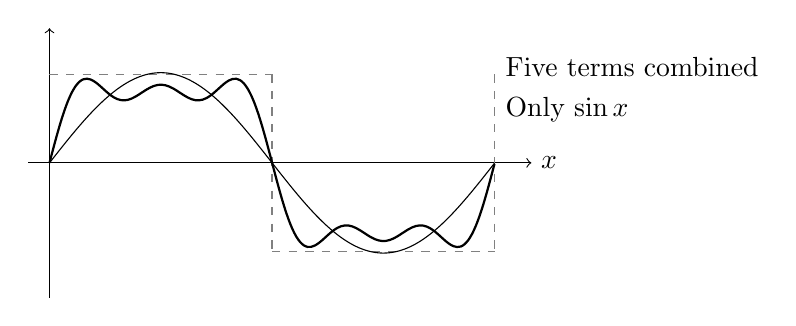
\begin{tikzpicture}[scale=0.9]
  \draw[->] (-0.3,0) -- (6.8,0) node[right] {$x$};
  \draw[->] (0,-1.9) -- (0,1.9);
  \draw[gray,dashed] (0,1.25) -- (3.14,1.25) (3.14,-1.25) -- (6.28,-1.25);
  \draw[gray,dashed] (3.14,1.25) -- (3.14,-1.25) (6.28,1.25) -- (6.28,-1.25);
  \draw[domain=0:6.28,samples=80,smooth] plot (\x, {1.273*sin(\x r)});
  \draw[thick,domain=0:6.28,samples=120,smooth] plot (\x, {1.273*(sin(\x r)+sin(3*\x r)/3+sin(5*\x r)/5)});
  \node[right] at (6.3,1.35) {Five terms combined};
  \node[right] at (6.3,0.75) {Only $\sin x$};
\end{tikzpicture}
\end{center}

Substitute a particular value for an enduring surprise. At $x=\pi/2$, the square wave equals $1$, while $\sin(\pi/2)=1$, $\sin(3\pi/2)=-1$, and $\sin(5\pi/2)=1$ alternate in sign. Thus
\[
1=\frac{4}{\pi}\left(1-\frac13+\frac15-\frac17+\cdots\right),
\quad\text{so}\quad
\frac{\pi}{4}=1-\frac13+\frac15-\frac17+\cdots .
\]
$\pi$, hiding in a circle's circumference, can be calculated by alternating reciprocals of all odd numbers. After $100$ terms you get about two decimal places of $\pi$. Convergence is slow, but the identity is beautiful.

\begin{shiyan}
\textbf{Build a Square Wave by Hand.} On squared paper, draw $y=\sin x$ for $x$ from $0$ to $2\pi$, calculating points at $x=0, 0.5, 1, \dots$. Draw $\frac{1}{3}\sin 3x$, with triple frequency and one-third height. \textbf{Add} their heights at each $x$ and plot the new curve. Peaks flatten and troughs rise, revealing the beginnings of a rectangle. If you wish, add $\frac{1}{5}\sin 5x$. Three colours on one graph recreate Fourier's view two centuries ago.

\textbf{Another Experiment}: hum a sustained note into a phone spectrum app or music equalizer. Several bars appear: the lowest, brightest one is the fundamental, with overtones above. Your voice and a piano playing the same note sound different because their overtone bars have different relative heights. Timbre is written in Fourier coefficients.
\end{shiyan}

\begin{lianjie}
Fourier series live in your pocket. Music compression such as MP3 divides sound into short segments, decomposes each into frequency components, and discards inaudible high-frequency contributions, reducing data with little audible change. JPEG uses the related cosine transform: low-frequency coefficients describe smoothly varying regions, while details need high frequencies. Telephone noise reduction, seismic analysis, and medical imaging are descendants of Fourier's idea. A once-ridiculed claim now handles humanity's images and sounds daily.
\end{lianjie}

\section{The Complex Plane and Euler's Formula}

The third tool comes from our old friend $i$, with $i^2=-1$. You may have regarded $i$ as a temporary helper brought in to solve quadratics. Joined with analysis, it produces one of mathematics' most celebrated formulas.

Place complex numbers in the plane: $a+bi$ has horizontal coordinate $a$ and vertical coordinate $b$. Addition is vector translation. Multiplication is more surprising: multiplying by $i$ means \textbf{rotating ninety degrees anticlockwise}. Multiplying $1$ by $i$ gives $i$, moving $(1,0)$ to $(0,1)$; another multiplication by $i$ gives $-1$, another ninety-degree turn. Two turns give a half-turn, or multiplication by $-1$. Geometrically, $i^2=-1$ says two quarter-turns make a half-turn. Complex multiplication is \textbf{rotation combined with scaling}.

Now invite power series in. Euler tried something apparently wild: insert the purely imaginary $i\theta$ into the recipe for $e^x$. The cycle $i^2=-1$, $i^3=-i$, $i^4=1$ separates odd and even terms into two teams:
\[
e^{i\theta}=\left(1-\frac{\theta^2}{2!}+\frac{\theta^4}{4!}-\cdots\right)
+i\left(\theta-\frac{\theta^3}{3!}+\frac{\theta^5}{5!}-\cdots\right).
\]
The bracketed series are precisely the recipes for $\cos\theta$ and $\sin\theta$, checkable using Chapter 10's derivatives: all derivative values at $0$ match. Thus:

\begin{dingli}[Euler's Formula]
For every real $\theta$,
\[
e^{i\theta}=\cos\theta+i\sin\theta .
\]
\end{dingli}

Its geometry is breathtaking. The right side is the unit-circle point at angle $\theta$; the left is $e$ raised to a purely imaginary power. As $\theta$ increases, $e^{i\theta}$ moves uniformly around the unit circle. Set $\theta=\pi$: since $\cos\pi=-1$ and $\sin\pi=0$,
\[
e^{i\pi}+1=0 .
\]
Five fundamental constants---$0$, $1$, $\pi$, $e$, and $i$---stand together, joined by addition, multiplication, and exponentiation. This identity rarely misses a mathematician's list of the most beautiful formulas.

\begin{center}
\begin{tikzpicture}[scale=1.6]
  \draw[->] (-1.6,0) -- (1.8,0) node[right] {Real axis};
  \draw[->] (0,-1.6) -- (0,1.8) node[above] {Imaginary axis};
  \draw (0,0) circle (1);
  \draw[->,thick] (0,0) -- (0.5,0.866);
  \fill (0.5,0.866) circle (1pt) node[above right] {$e^{i\theta}$};
  \draw (0.28,0) arc (0:60:0.28) node[midway,right] {$\theta$};
  \fill (-1,0) circle (1pt) node[below left] {$-1=e^{i\pi}$};
  \fill (1,0) circle (1pt) node[below right] {$1$};
  \fill (0,1) circle (1pt) node[above left] {$i$};
\end{tikzpicture}
\end{center}

Euler's formula is also Fourier series' official language. With $\cos\theta=\frac{e^{i\theta}+e^{-i\theta}}{2}$ and $\sin\theta=\frac{e^{i\theta}-e^{-i\theta}}{2i}$, sums of sines and cosines become sums of $e^{ik\theta}$, turning trigonometric identities into simple exponent arithmetic. Engineers doing Fourier analysis often write scarcely any $\sin$ or $\cos$, instead using rotating arrows $e^{i\theta}$.

One step farther lies \textbf{complex analysis}: replace $x$ with complex $z$ and study $f(z)$. Something extraordinary happens. Complex differentiability is so strong that a function differentiable throughout a region is automatically smooth, automatically has power-series expansions, and has its values fixed by boundary values. It resembles a red-hot metal plate where disturbing one part affects the whole. This rigidity makes complex analysis elegant and powerful, and leads to some of mathematics' deepest questions.

\section{What We Have Gained}

\begin{toolbox}
This chapter's new tools:

\begin{itemize}
  \item \textbf{Continuity, intuitively}: you choose an error requirement, I supply a response. Close enough inputs give close enough outputs.
  \item \textbf{Completeness of the reals}: Cauchy sequences, whose later terms cluster, have real limits. The rationals lack this property.
  \item \textbf{The intermediate value theorem}: continuous functions take every value between their endpoint values. Bisection both proves this and approximates zeros.
  \item \textbf{The extreme value theorem}: a continuous function on a closed interval attains maximum and minimum; neither hypothesis can be dropped.
  \item \textbf{Uniform continuity}: one response works throughout the interval. Continuous functions on closed intervals have it.
  \item \textbf{Power series}: infinitely long polynomial recipes, such as $e^x=\sum x^n/n!$, each with its own convergence radius.
  \item \textbf{Fourier series}: periodic functions as sums of sine waves; the square-wave expansion also yields $\pi/4=1-1/3+1/5-\cdots$.
  \item \textbf{Euler's formula}: $e^{i\theta}=\cos\theta+i\sin\theta$, expressing complex multiplication as rotation and scaling, with special case $e^{i\pi}+1=0$.
\end{itemize}
\end{toolbox}

\begin{pandeng}
Signposts for further climbing:

\begin{itemize}
  \item \textbf{$\varepsilon$--$\delta$ language}: our challenge-and-response agreement in precise symbols, the first lesson of university analysis.
  \item \textbf{The Weierstrass function}: an everywhere-continuous, nowhere-differentiable bristly curve, rigorously constructed using a uniformly convergent series of functions.
  \item \textbf{Taylor series}: the general theory of power-series recipes, with coefficients determined by successive derivatives.
  \item \textbf{The fast Fourier transform (FFT)}: an algorithm dramatically reducing the work of Fourier decomposition, often counted among the twentieth century's most important algorithms.
  \item \textbf{The Riemann $\zeta$ function and Riemann hypothesis}: a jewel of complex analysis connecting our series to next chapter's primes, and an unsolved million-dollar problem.
\end{itemize}
\end{pandeng}

\section*{Questions to Think About}

\textbf{Observation}
\begin{sikao}
  \item One day you climb from foot to summit between $12$ noon and $4$ p.m.; the next day you descend the same route between $12$ noon and $4$ p.m. Use the intermediate value theorem to prove that at some clock time on both days you are at the same altitude. \emph{Hint}: plot both altitude functions together and consider their difference.
  \item Does $x^3+x-1=0$ have a solution between $0$ and $1$? Perform three bisections by hand to narrow its location to an interval of length $1/8$. \emph{Hint}: evaluate at $x=0,\frac12,1$, then halve.
\end{sikao}

\textbf{Proof}
\begin{sikao}
  \setcounter{sikaoi}{2}
  \item Prove that a continuous $f$ satisfying $f(a)\cdot f(b)<0$ has a zero in $(a,b)$, the intermediate value theorem. Complete the bisection proof's explanation that nondecreasing, bounded left endpoints approach some $c$. \emph{Hint}: what happens to a sequence moving steadily rightward without ever passing a wall?
  \item For $a_n=\frac{n}{n+1}$, or $\frac12,\frac23,\frac34,\dots$, verify the Cauchy property. How small is $|a_m-a_n|$ when $m,n$ both exceed some $N$? \emph{Hint}: $|a_m-a_n|=\left|\frac{1}{n+1}-\frac{1}{m+1}\right|$; bound each fraction separately.
\end{sikao}

\textbf{Challenge}
\begin{sikao}
  \setcounter{sikaoi}{4}
  \item Use $e^{i\theta}=\cos\theta+i\sin\theta$ to calculate $e^{i\alpha}\cdot e^{i\beta}$. Expand once using exponent laws and once using complex multiplication, then compare real and imaginary parts. Which two trigonometric identities emerge for free? \emph{Hint}: what is the real part after expanding $(\cos\alpha+i\sin\alpha)(\cos\beta+i\sin\beta)$?
  \item The series $1-\frac13+\frac15-\frac17+\cdots$ converges slowly to $\pi/4$. Approximately how large is the error after $100$ terms? Estimate by comparing consecutive partial sums. \emph{Hint}: alternating partial sums fall on opposite sides of the limit, with error bounded by the first omitted term.
\end{sikao}

\section*{The Door to the Next Chapter}

End with one suggestive look at the harmonic series:
\[
1+\frac12+\frac13+\frac14+\frac15+\cdots .
\]
Its terms tend to $0$, but its sum \textbf{grows without bound}. Grouping gives $\frac13+\frac14>\frac12$, $\frac15+\frac16+\frac17+\frac18>\frac12$, and the eight terms from $\frac19$ to $\frac1{16}$ again exceed $\frac12$. Infinitely many halves make the sum unstoppable.

Euler asked a history-changing question about this small fact: what does harmonic divergence have to do with \textbf{prime numbers}? He found an astonishing identity: the sum of reciprocals of all positive integers equals an infinite product made only from primes. If there were only finitely many primes, the product would be finite, contradicting the divergent harmonic sum. Analysis thus reproved Euclid's two-thousand-year-old theorem of infinitely many primes, with a sharper tool.

Beyond this door lies a new world: integer multiplication and division hide series, functions, and even the complex plane. To read it, return first to simple questions. What are primes? What patterns govern them? Why is a factorization such as $7\times 11\times 13=1001$ unique? Next chapter we enter the world of integers, congruences, and the modern cryptography they protect.
